\documentclass[onecolumn,12pt]{IEEEtran}
\ifCLASSINFOpdf
	\usepackage[pdftex]{graphicx}
	\usepackage{epstopdf}
	\graphicspath{{./figures/}}
	\DeclareGraphicsExtensions{.pdf,.jpeg,.png,.eps}
\else
	\usepackage[dvips]{graphicx}
	\graphicspath{{./figures/}}
	\DeclareGraphicsExtensions{.eps}
\fi

\usepackage[caption=false,font=footnotesize]{subfig}
\usepackage{dblfloatfix}

\usepackage{url}
\linespread{1.5}
%\IEEEoverridecommandlockouts

% Title Page
\title{Desktop and Mobile Web Page Comparison: Characteristics, Trends, and Implications
	\thanks{T. Johnson and P.~Seeling are with the Dept.~of Computer Science,
		Central Michigan University, Mount Pleasant, MI 48859, Email: \texttt{johns4ta@cmich.edu,pseeling@ieee.org}}
}

\author{Troy Johnson and Patrick~Seeling
	\thanks{Please direct correspondence to P.~Seeling.}
	\thanks{Supported in part by an Early Career Grant from the Office of Research and Sponsored Programs at Central Michigan University.}
	\thanks{\textcopyright 20xx IEEE. Personal use of this material is permitted. Permission from IEEE must be obtained for all other uses, in any current or future media, including reprinting/republishing this material for advertising or promotional purposes, creating new collective works, for resale or redistribution to servers or lists, or reuse of any copyrighted component of this work in other works.}
}

\begin{document}



\section{Comparison of Desktop and Mobile Web Page Characteristics}
\label{s:compare}

\newpage
\subsection{Average Number of Web Site Objects}
\label{ss:objects}

\begin{figure}
\centering
	\subfloat[Average total number for desktop and mobile client versions.]{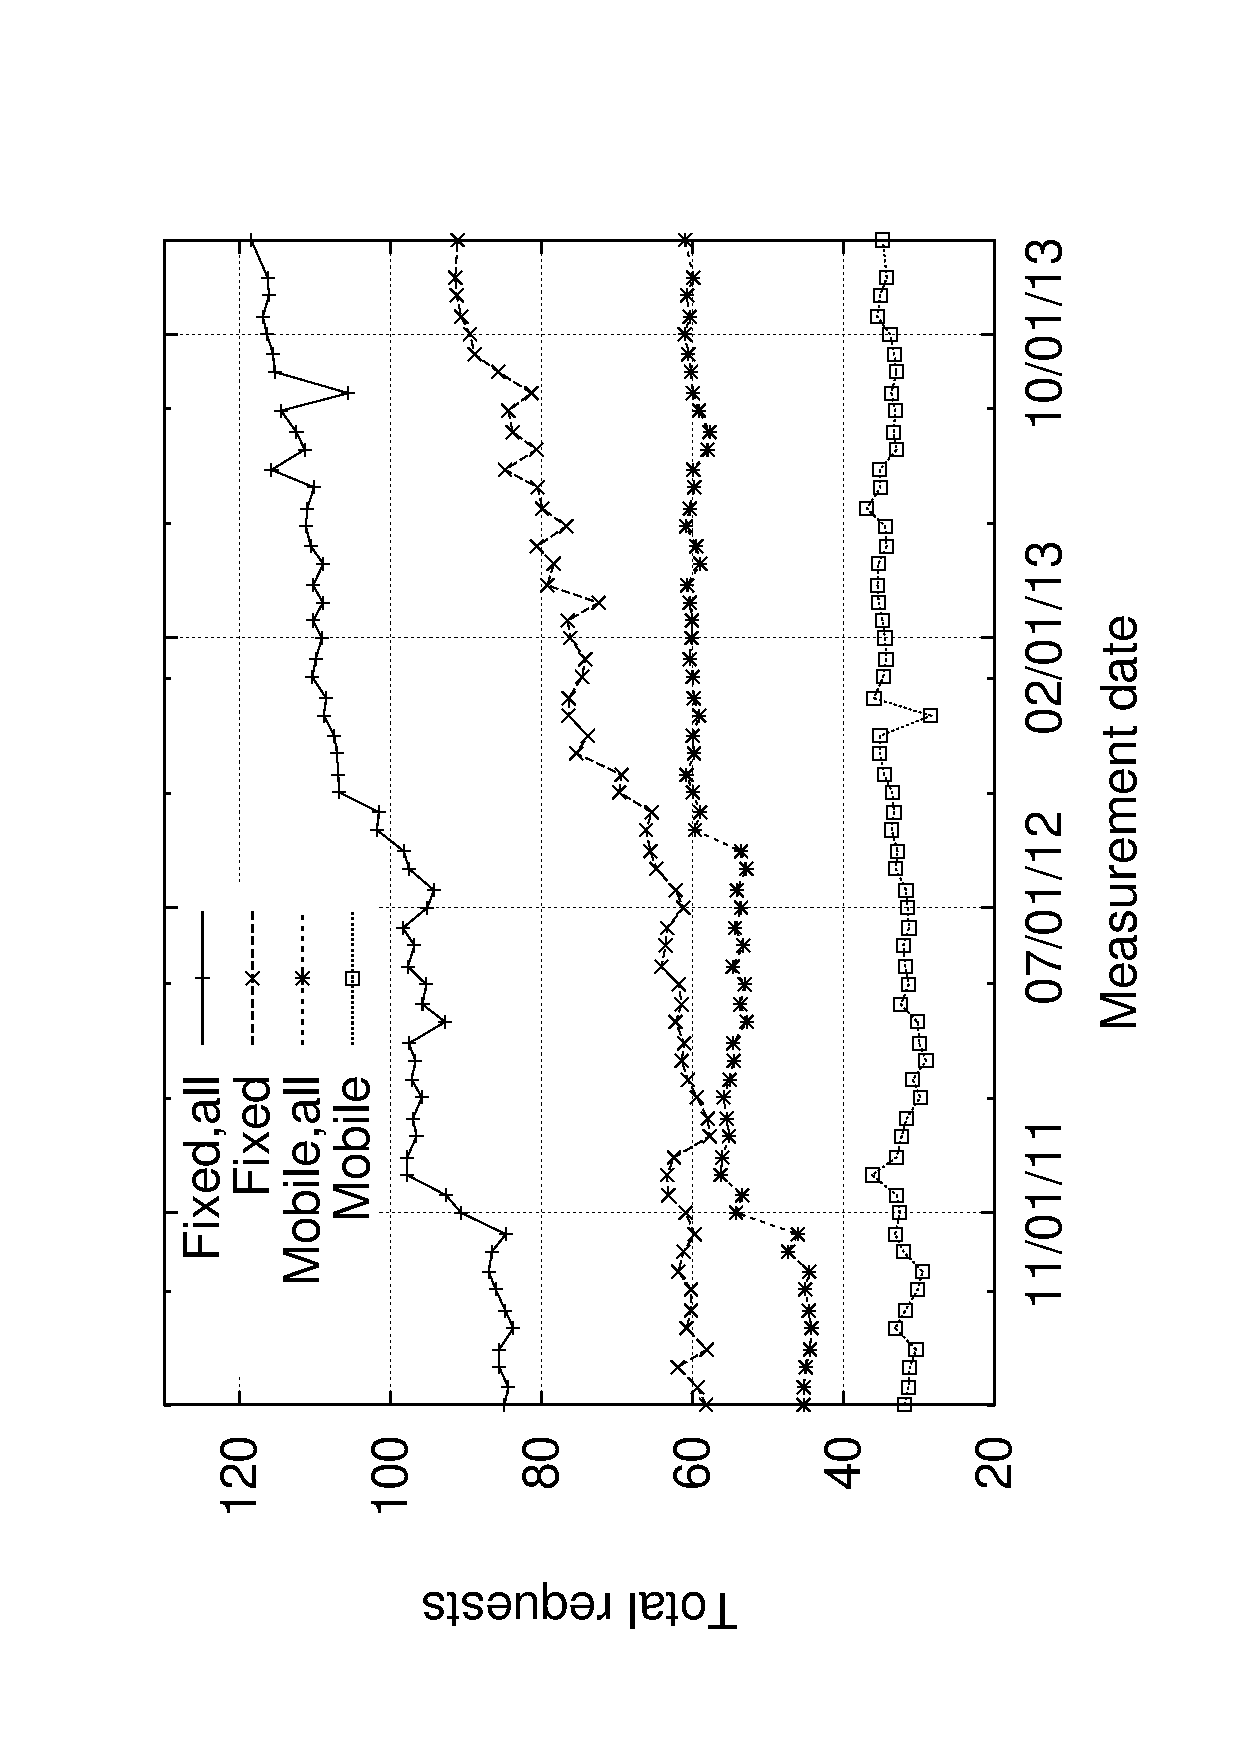
\includegraphics[angle=270,width=.5\textwidth]{totalRequests/totalRequests_all}}\\
	\subfloat[Average number by category for desktop client versions.]{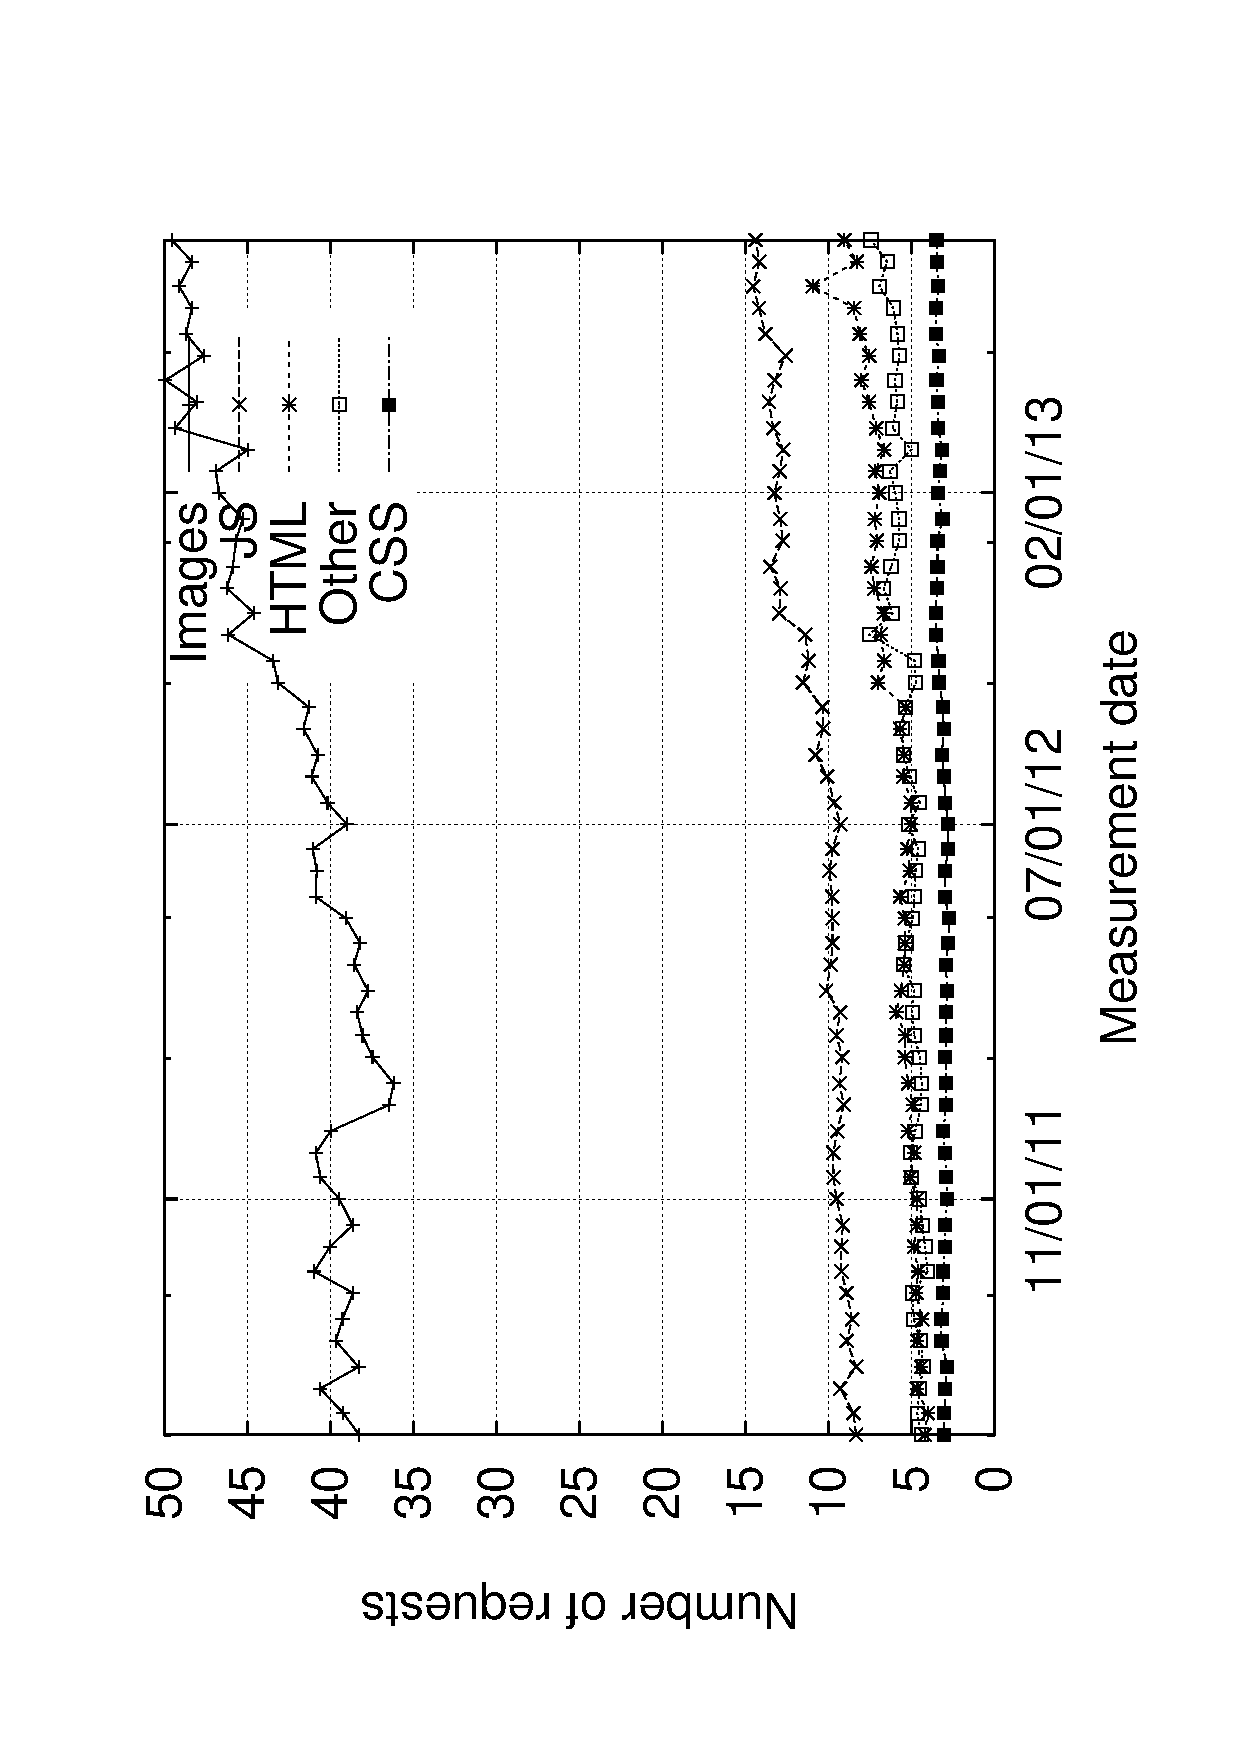
\includegraphics[angle=270,width=.5\textwidth]{requests_by_type/req_by_type_fixed}}\\
	\subfloat[Average number by category for mobile client versions.]{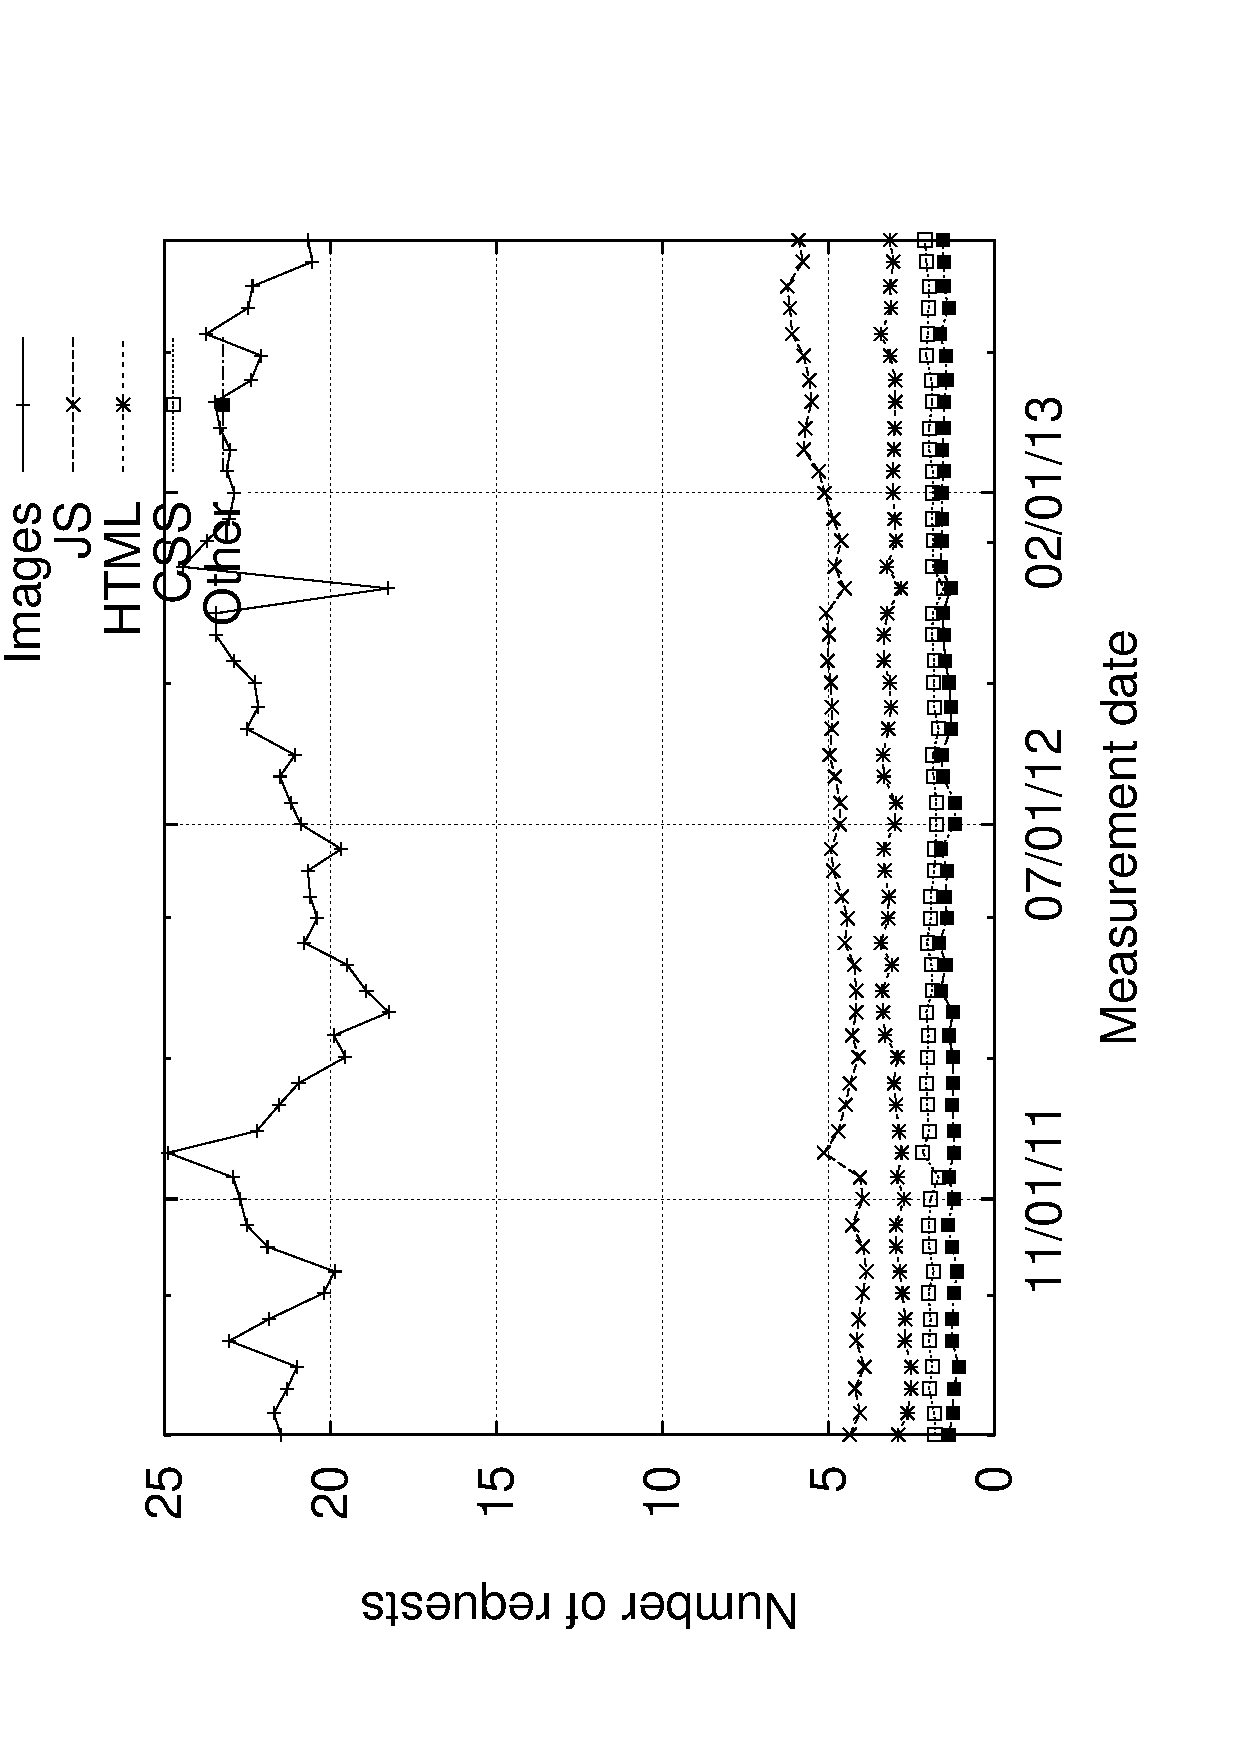
\includegraphics[angle=270,width=.5\textwidth]{requests_by_type/req_by_type_mobile}}\\
\caption{Average total number of requests for objects constituting a web page in desktop and mobile versions and decomposition into  HTML, CSS, Java Script, Images, and Other object categories.\label{fig:requests}}
\end{figure}


\newpage
\subsection{Average Web Page Sizes}
\label{ss:bytes}

\begin{figure}
	\centering
	\subfloat[Average total amount for desktop and mobile client versions.]{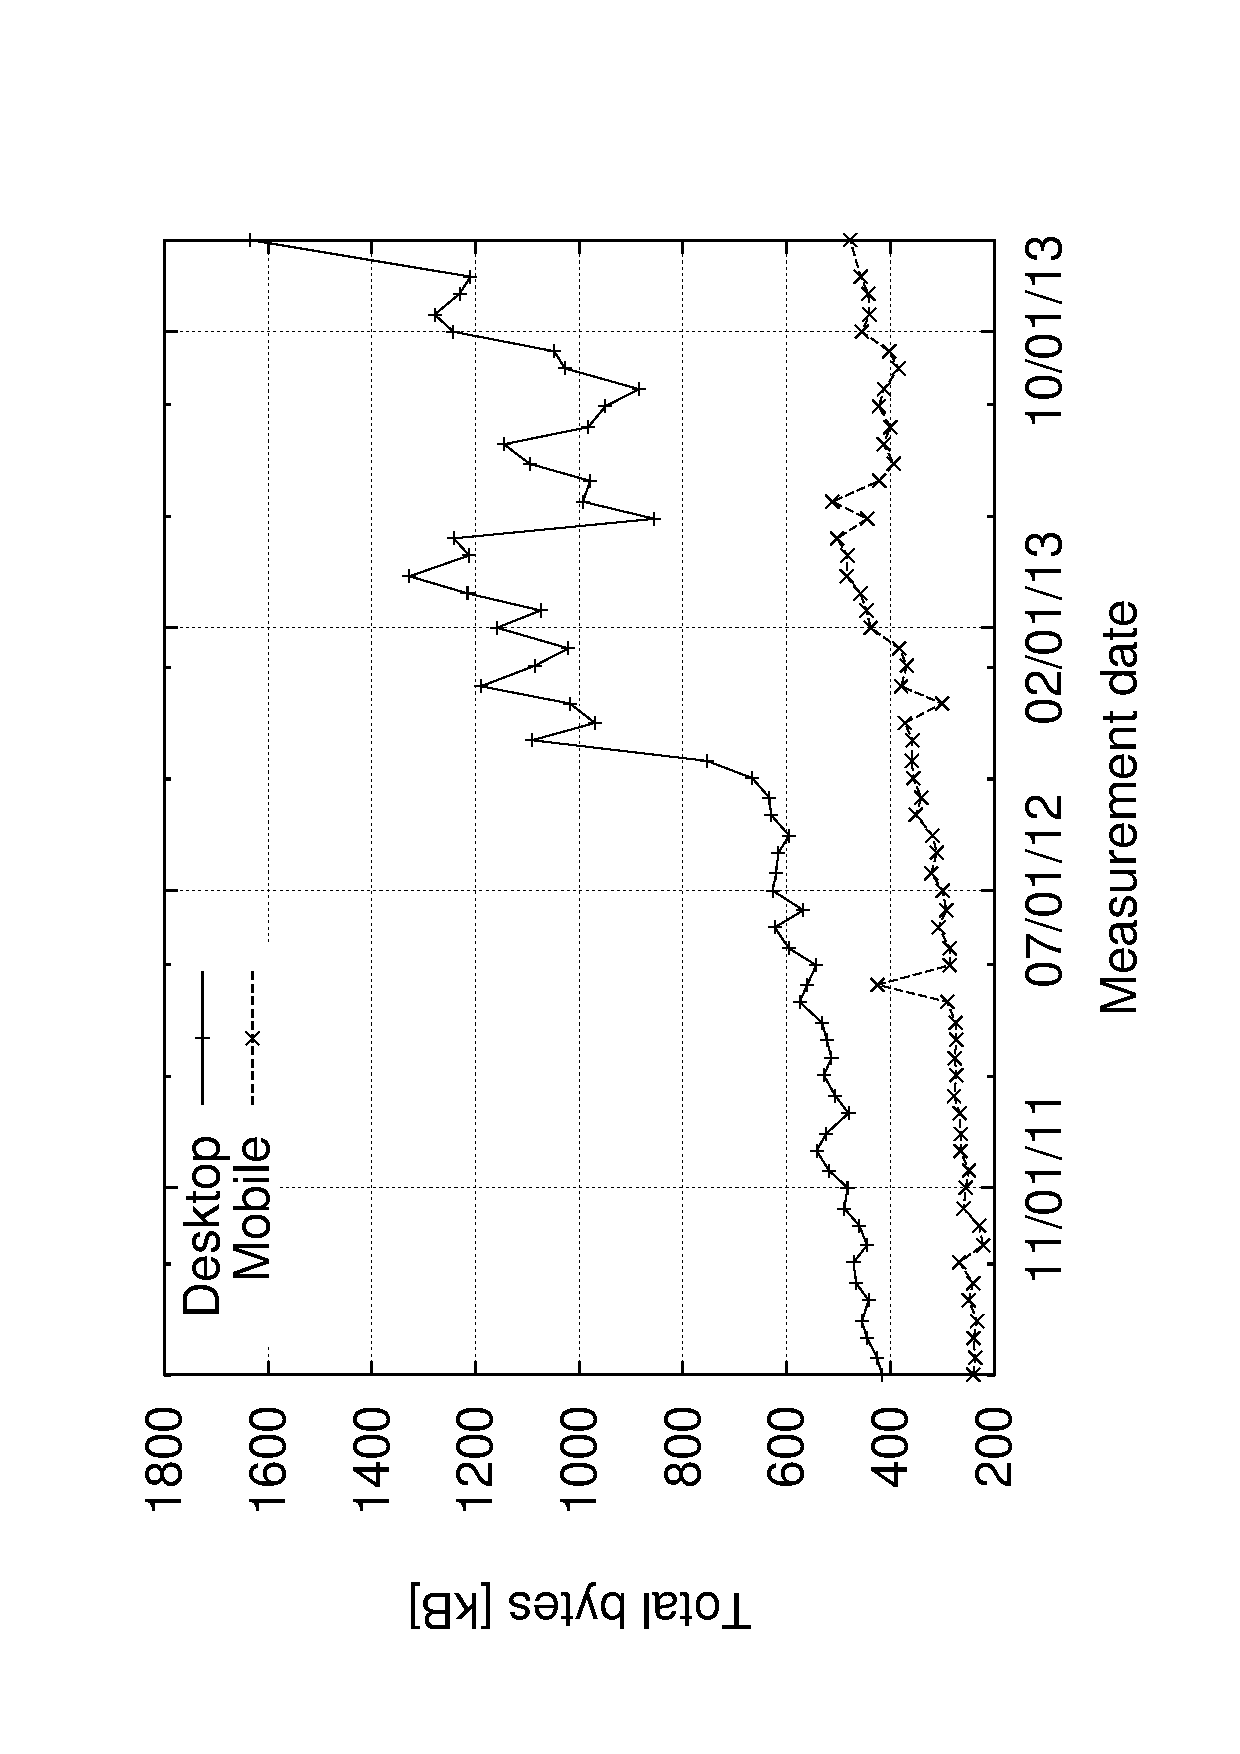
\includegraphics[angle=270,width=.57\textwidth]{bytes_total/bytes_total}}\\
	\subfloat[Average amount by category for desktop client versions.]{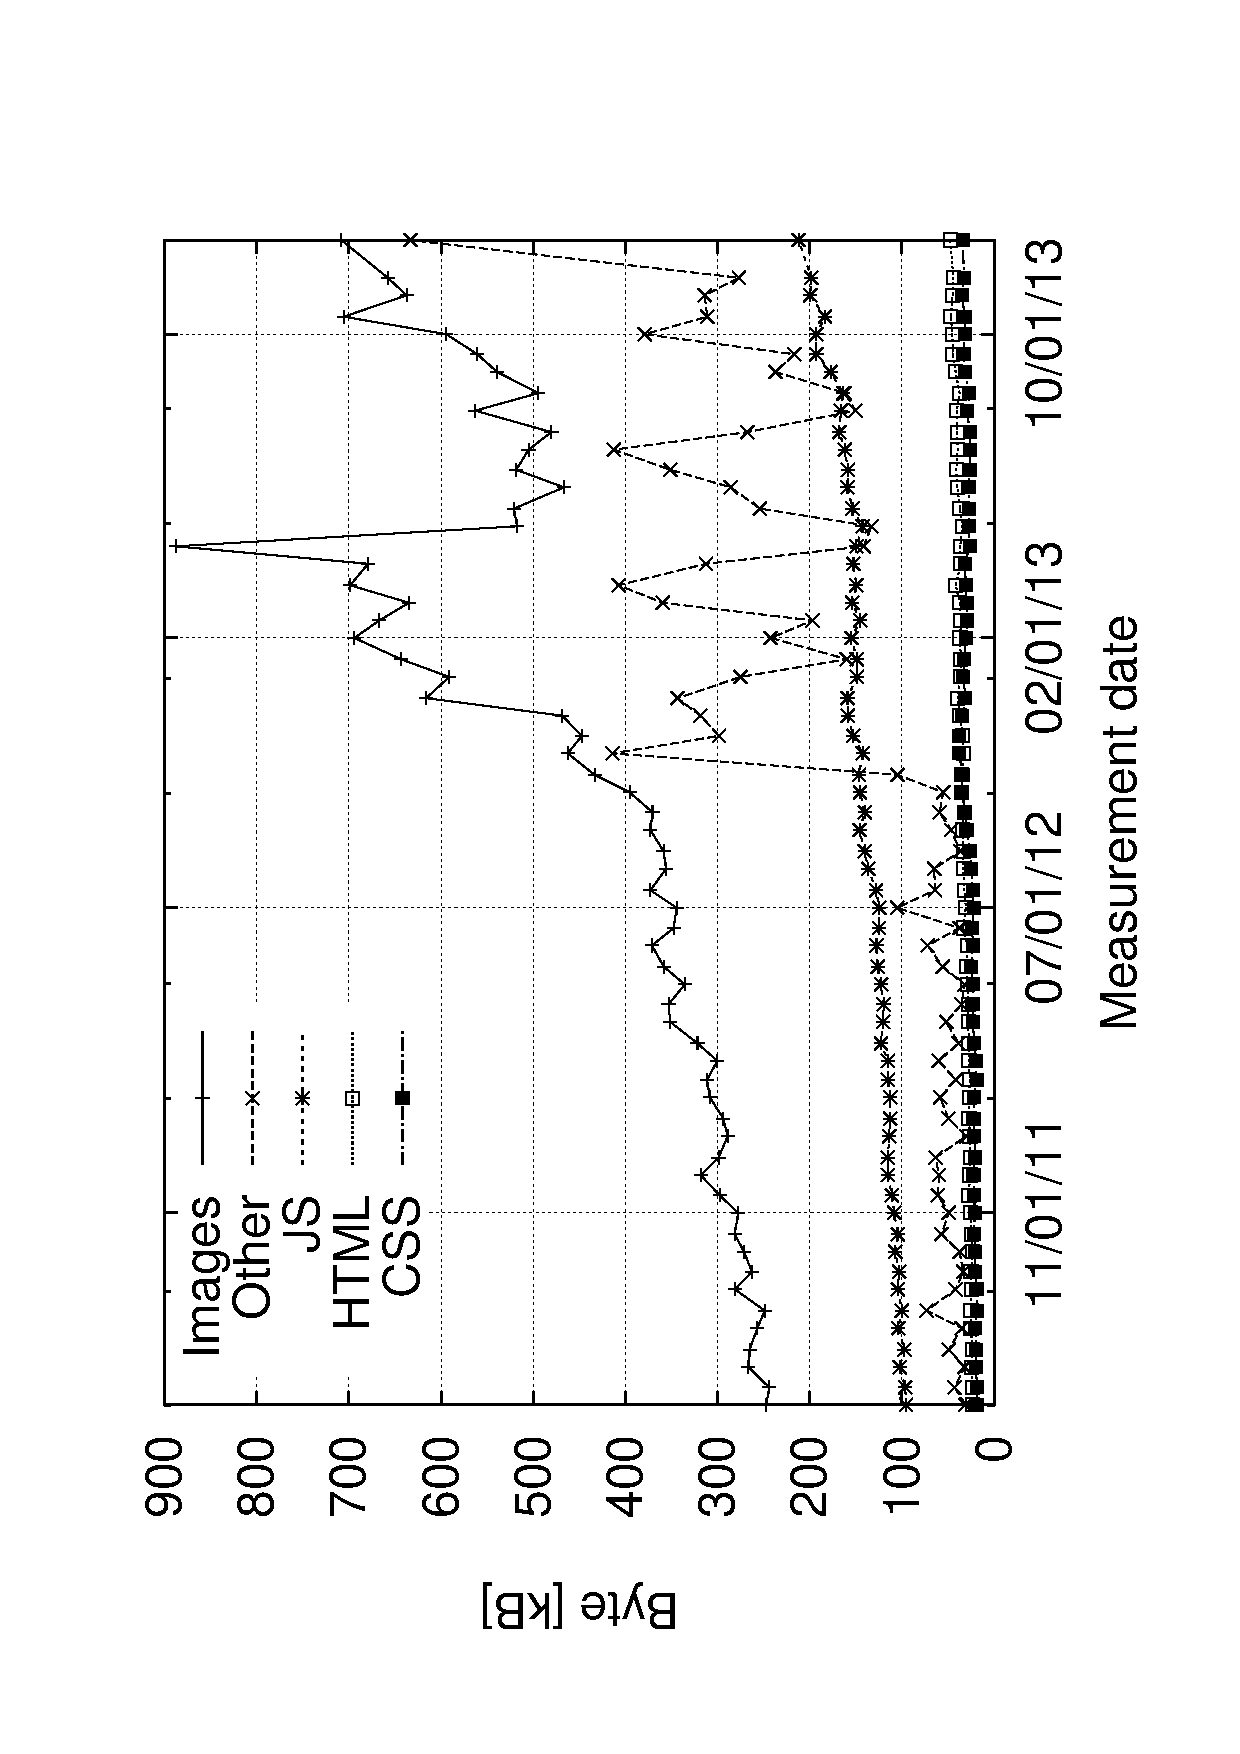
\includegraphics[angle=270,width=.57\textwidth]{bytes_by_type/bytes_by_type_fixed}}\\
	\subfloat[Average amount by category for mobile client versions.]{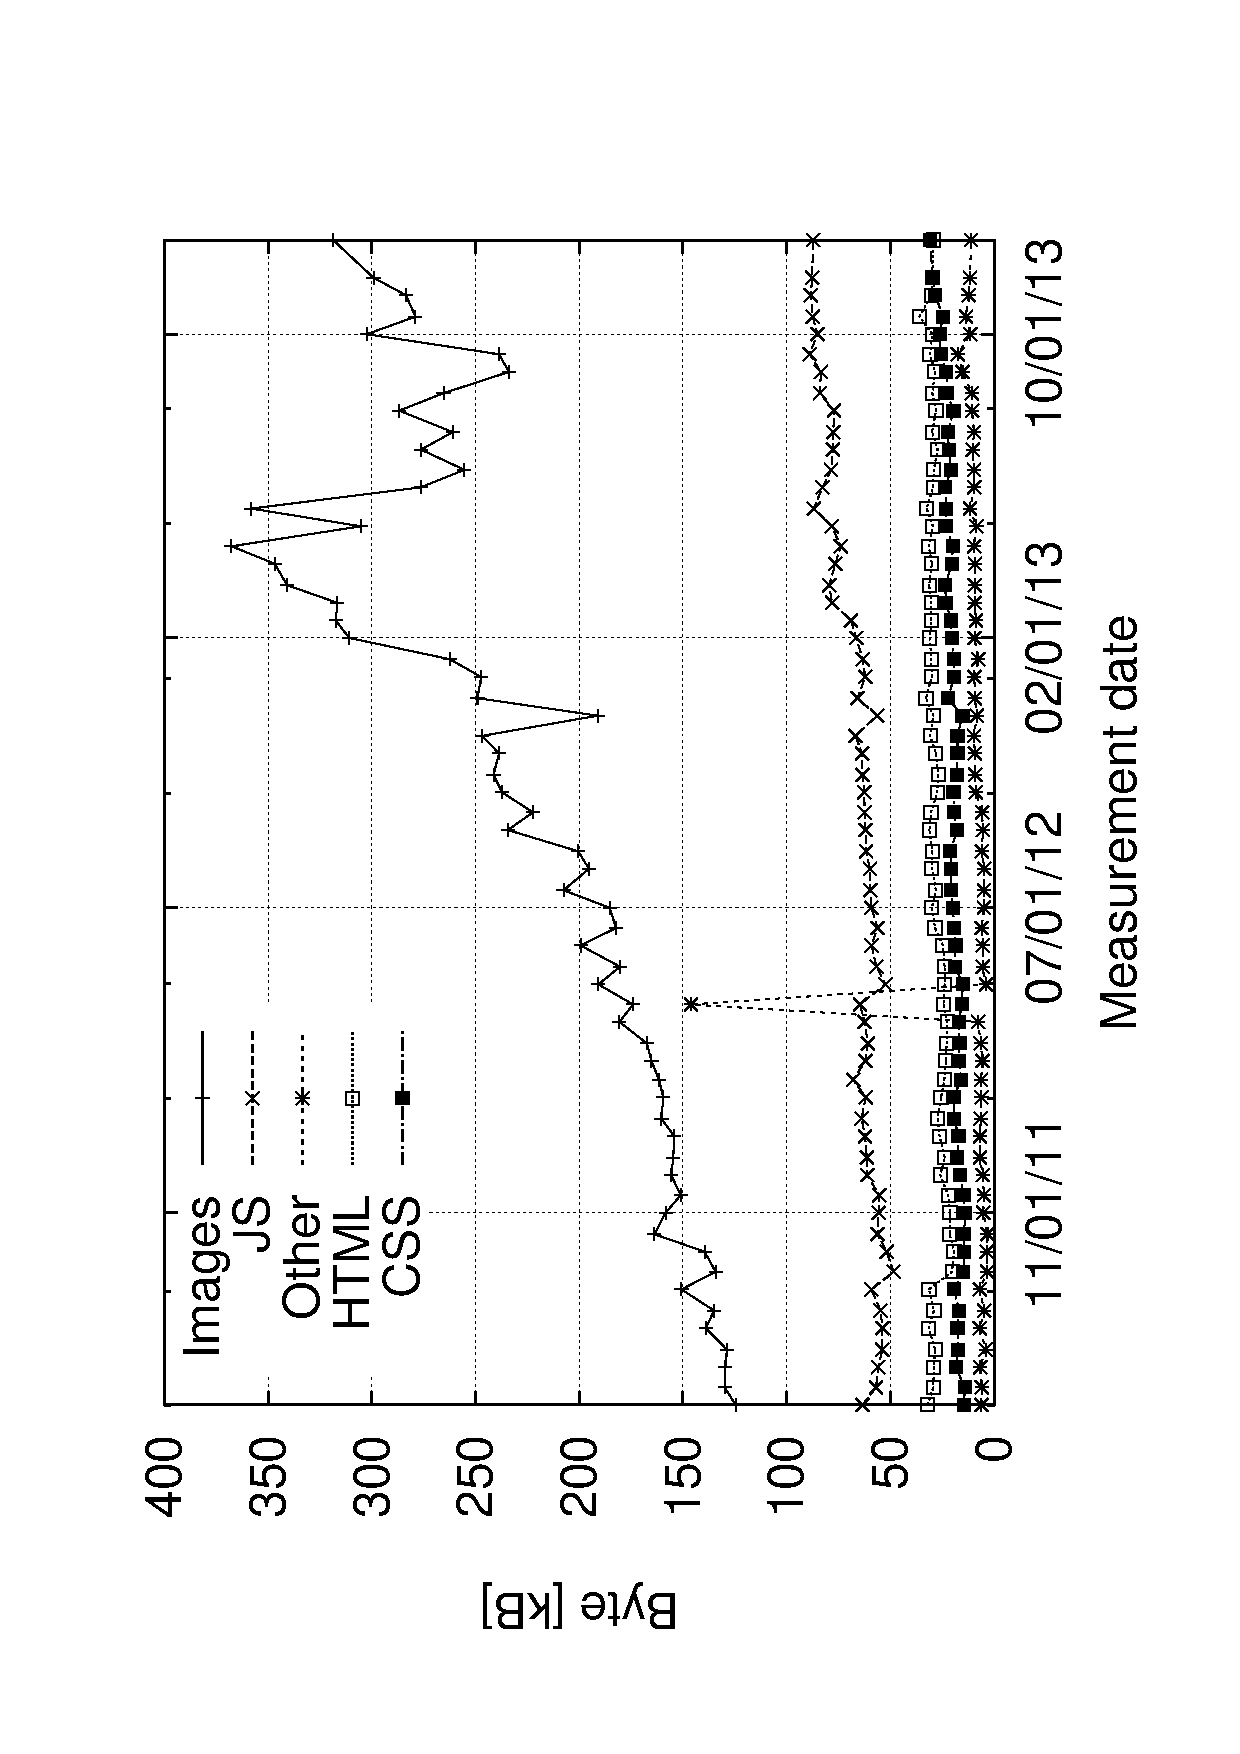
\includegraphics[angle=270,width=.57\textwidth]{bytes_by_type/bytes_by_type_mobile}}\\
	\caption{Average total number of bytes constituting a web page in desktop and mobile versions and decomposition into  HTML, CSS, Java Script, Images, and Other object categories.\label{fig:sizes}}
\end{figure}

\newpage
\subsection{Data per Web Page Object}

\begin{figure}
	\centering
	\subfloat[Average total amount for desktop and mobile client versions.]{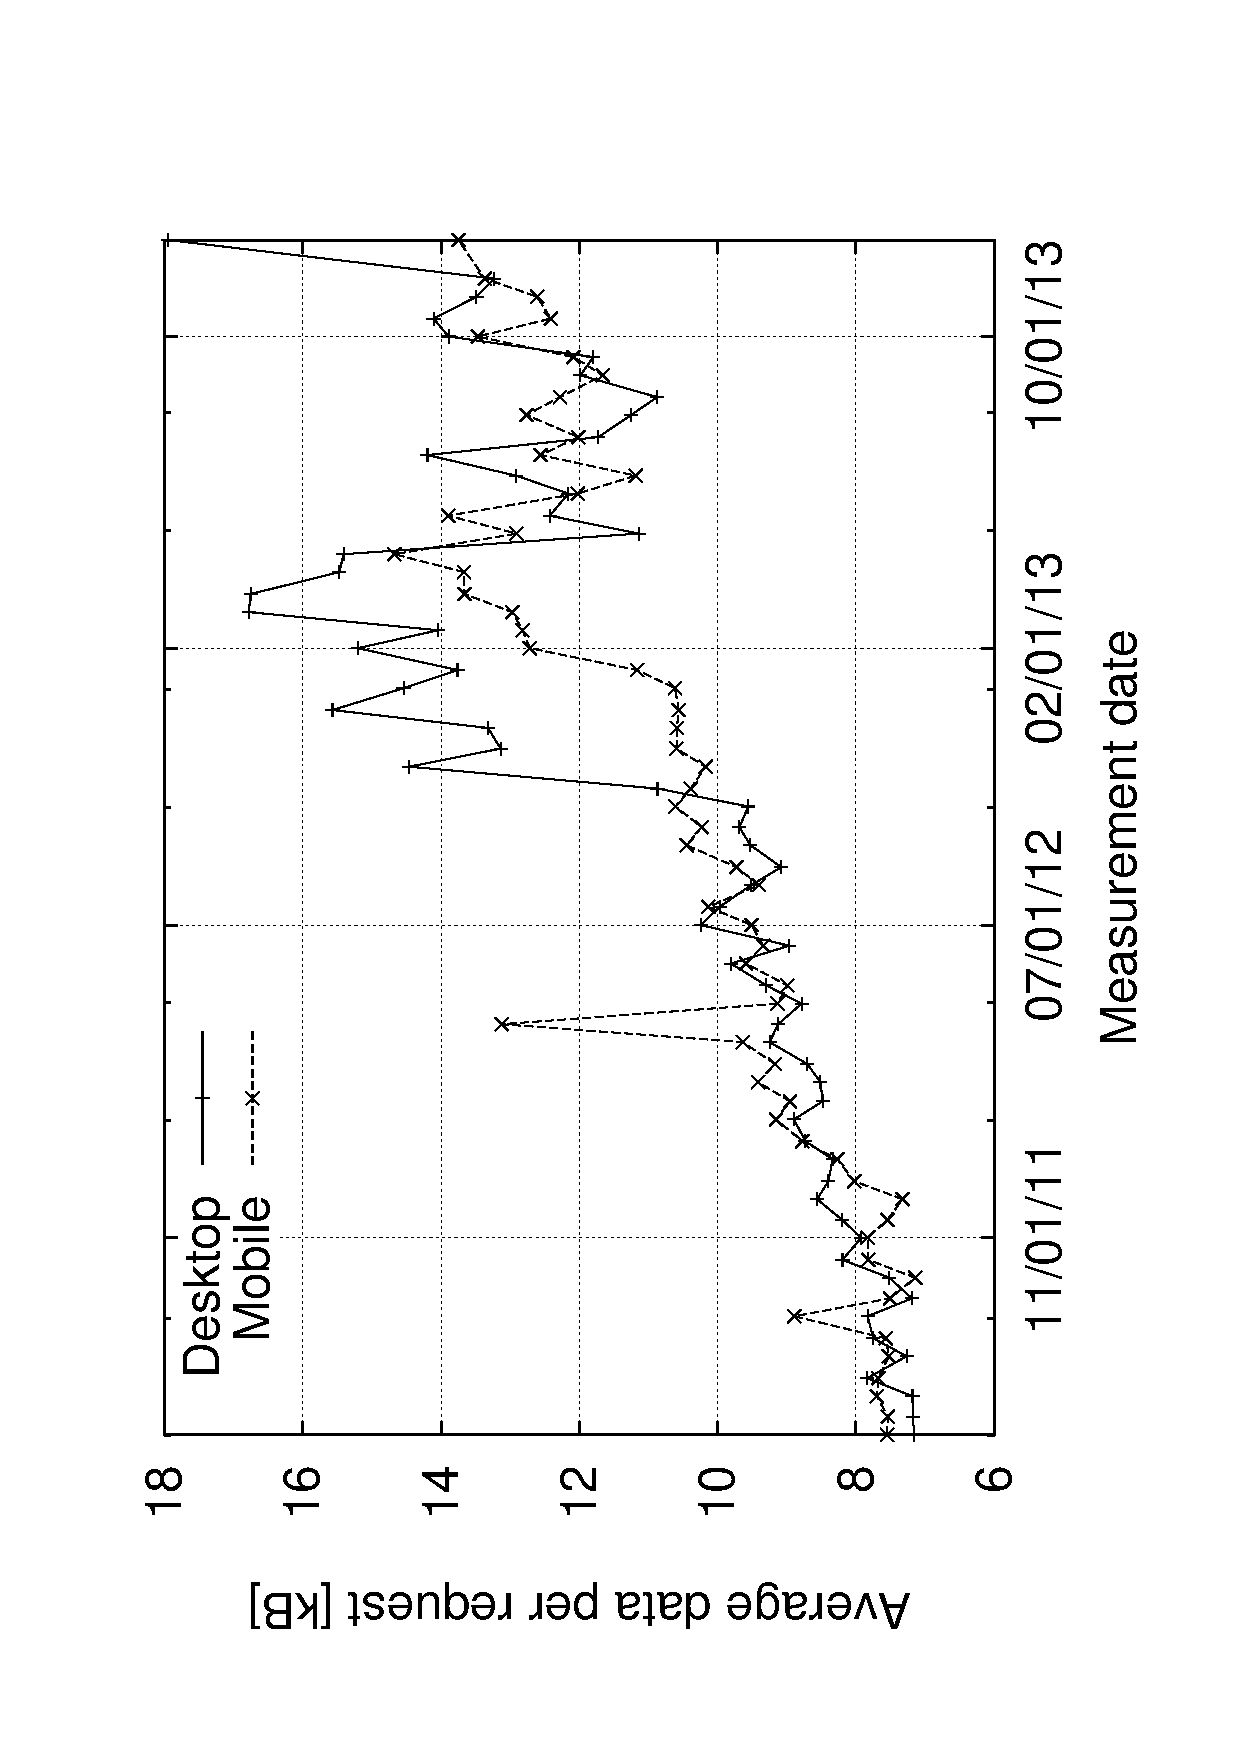
\includegraphics[angle=270,width=.57\textwidth]{bytes_per_request/bpr}}\\
	\subfloat[Average amount by category for desktop client versions.]{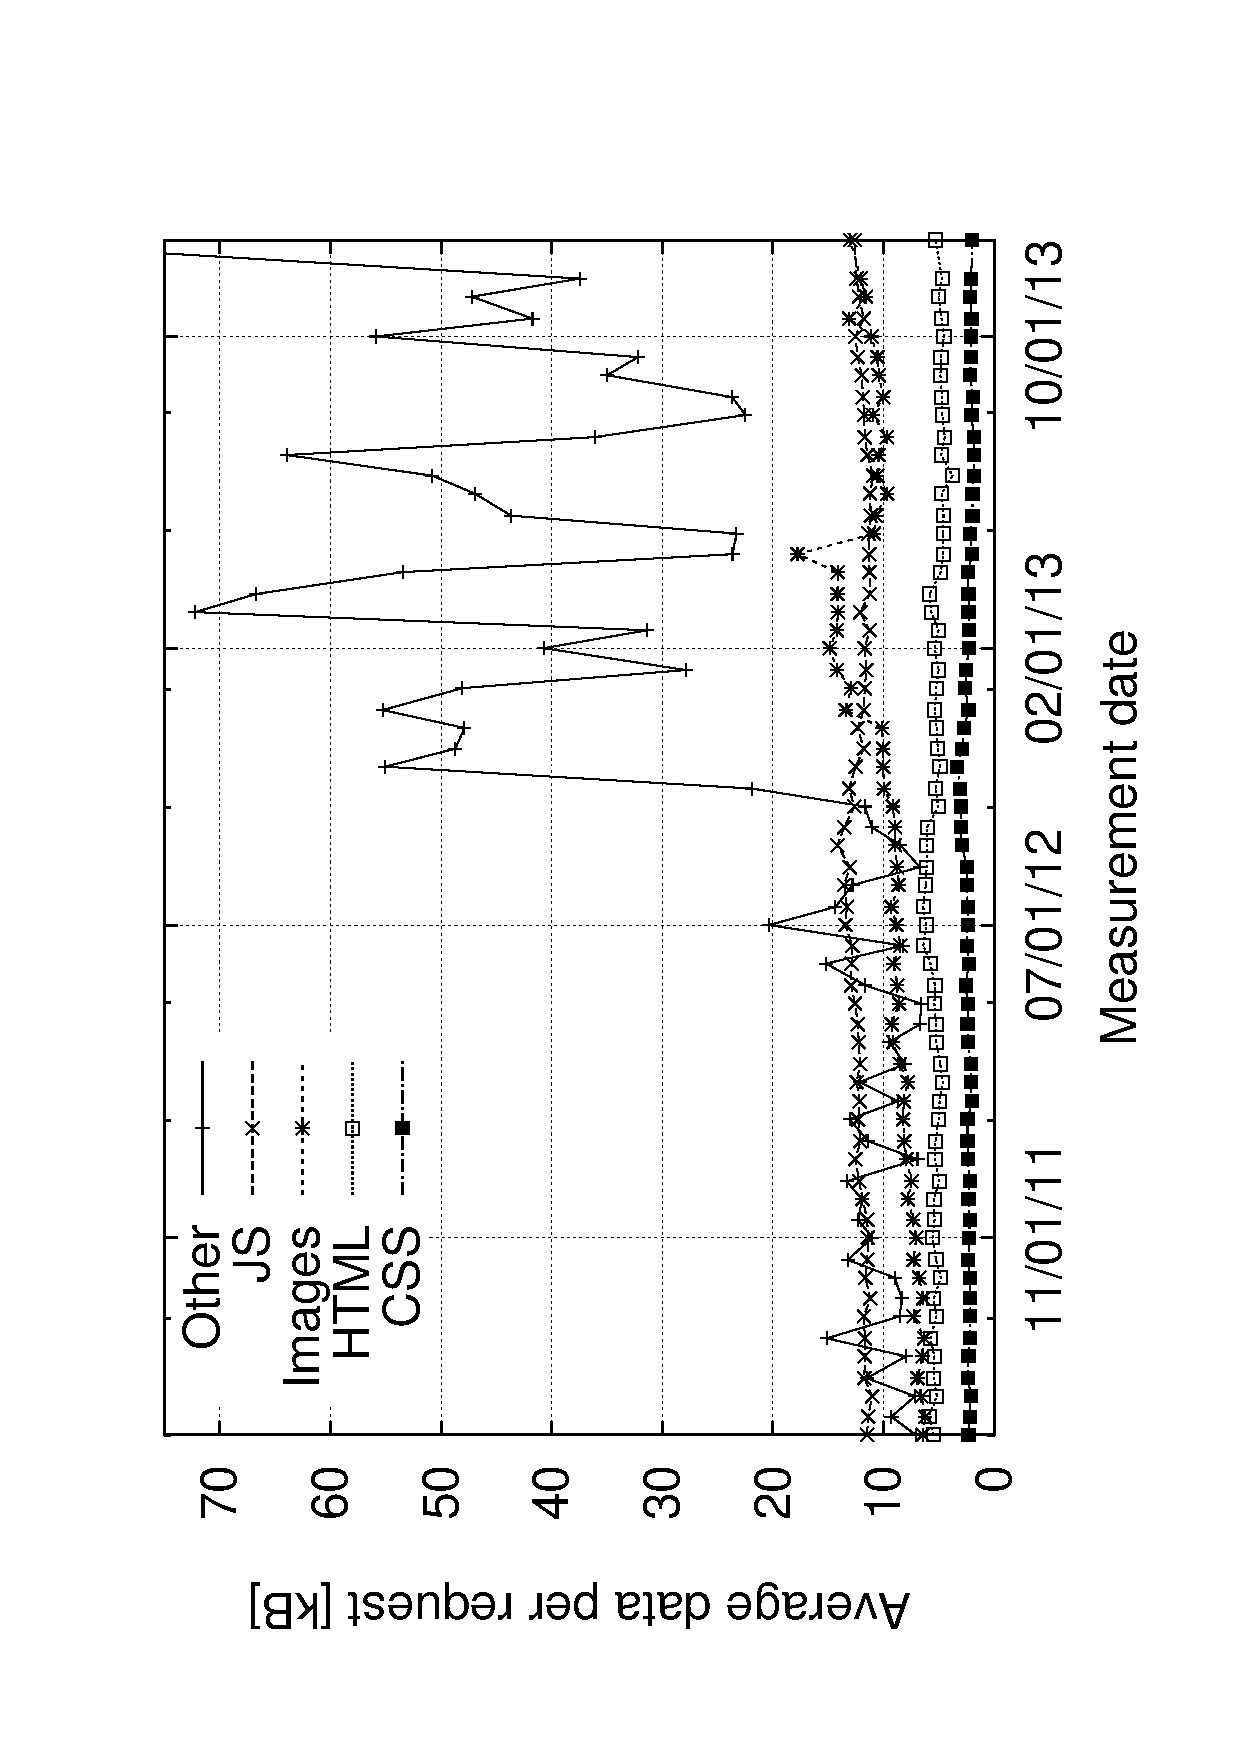
\includegraphics[angle=270,width=.57\textwidth]{bytes_per_request_by_type/bpr_by_type_fixed}}\\
	\subfloat[Average amount by category for mobile client versions.]{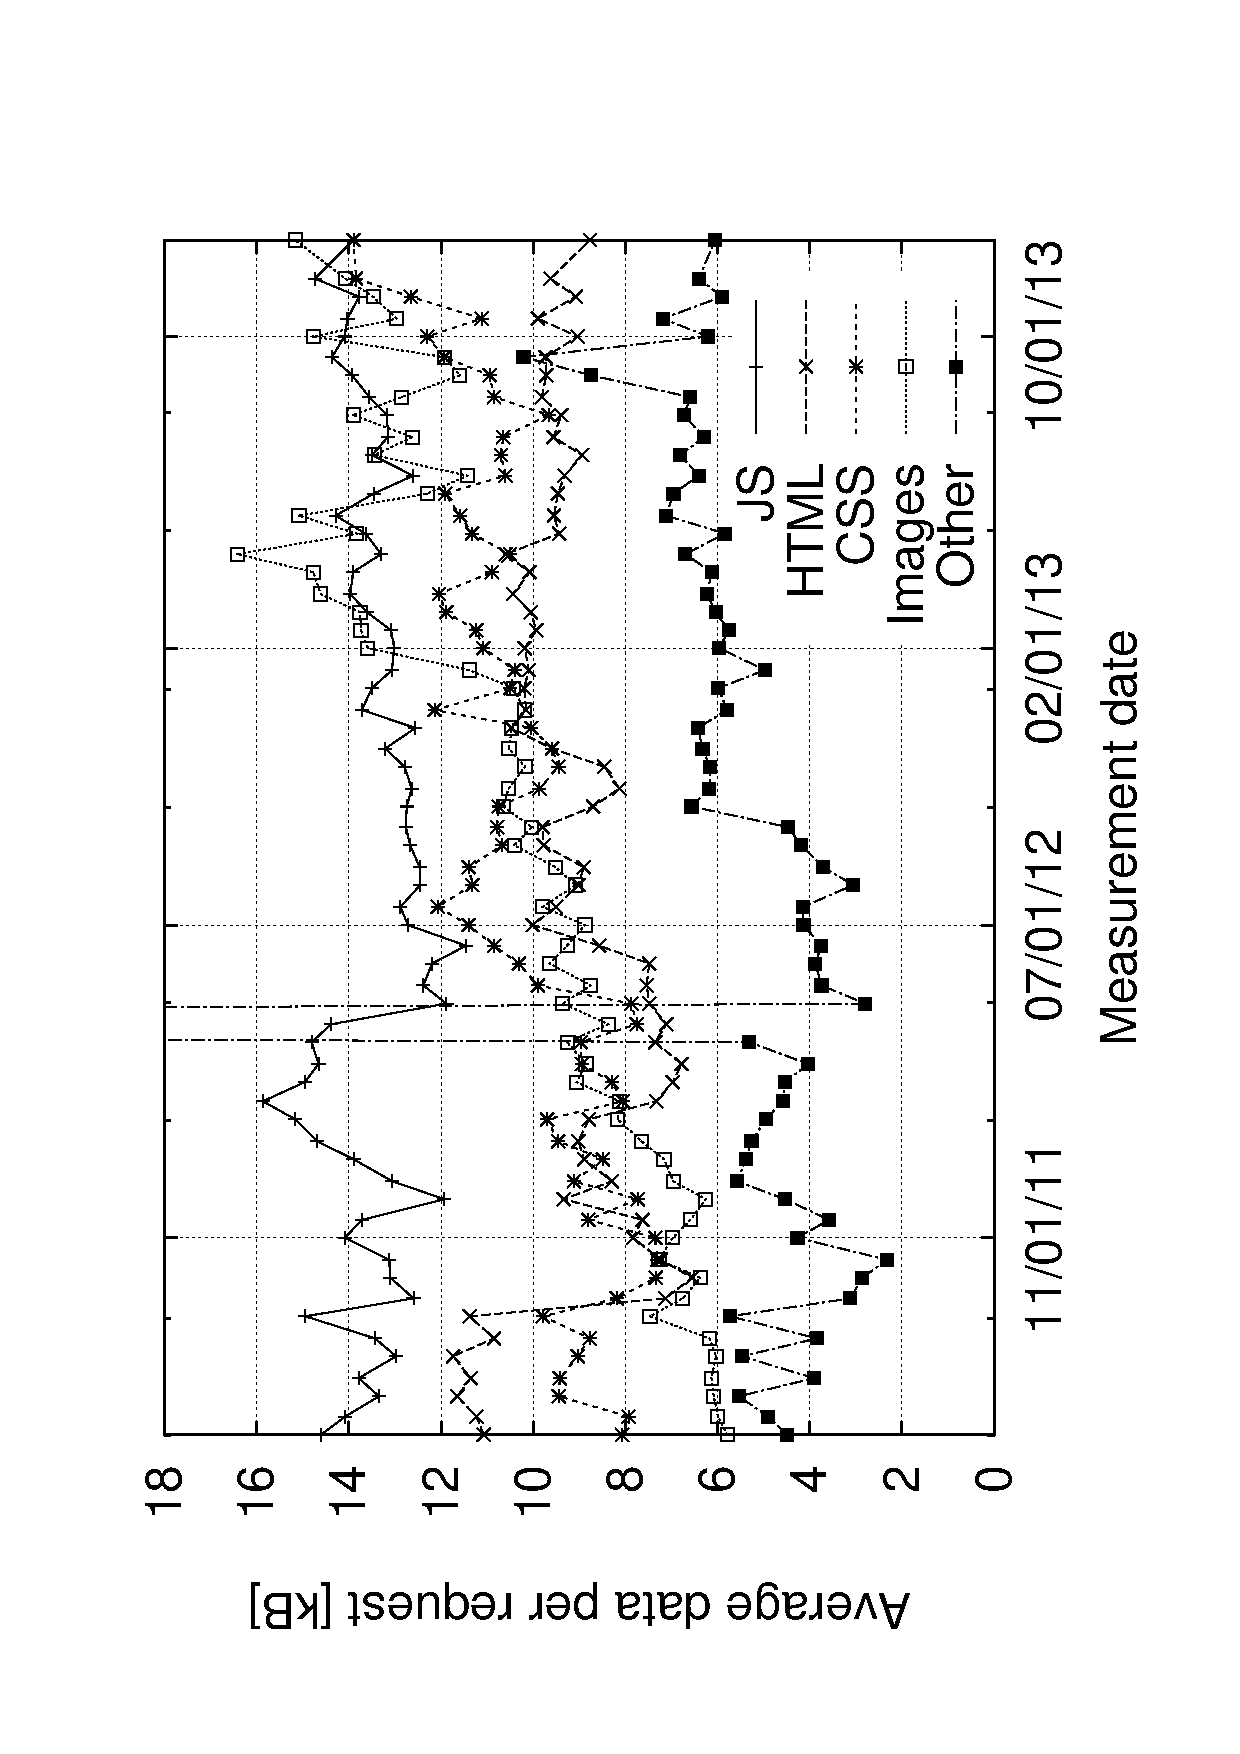
\includegraphics[angle=270,width=.57\textwidth]{bytes_per_request_by_type/bpr_by_type_mobile}}\\
	\caption{Average number of bytes per web page object request for desktop and mobile versions and decomposition into  HTML, CSS, Java Script, Images, and Other object categories.\label{fig:relative}}
\end{figure}

\newpage
\subsection{Caching of Web Page Objects}
One of the main assumptions for the prior evaluation was that the data represents ``first views,'' i.e., the dataset's underlying measurements do not consider the caching of web pages after initial visits. 
The individual entries in the datasets obtained from httparchive.org, however, additionally contain the max-age header (amongst other, such as expiration) directives for evaluation of the maximum lifetime of objects on the requesting device. The locally cached data can have a positive impact on the required network access, especially for mobile devices.

We illustrate the different max-age values obtained from the data in Figure~\ref{fig:maxage}~(a) for desktop client requests.
\begin{figure}
	\centering
 %	\subfloat[Desktop clients]{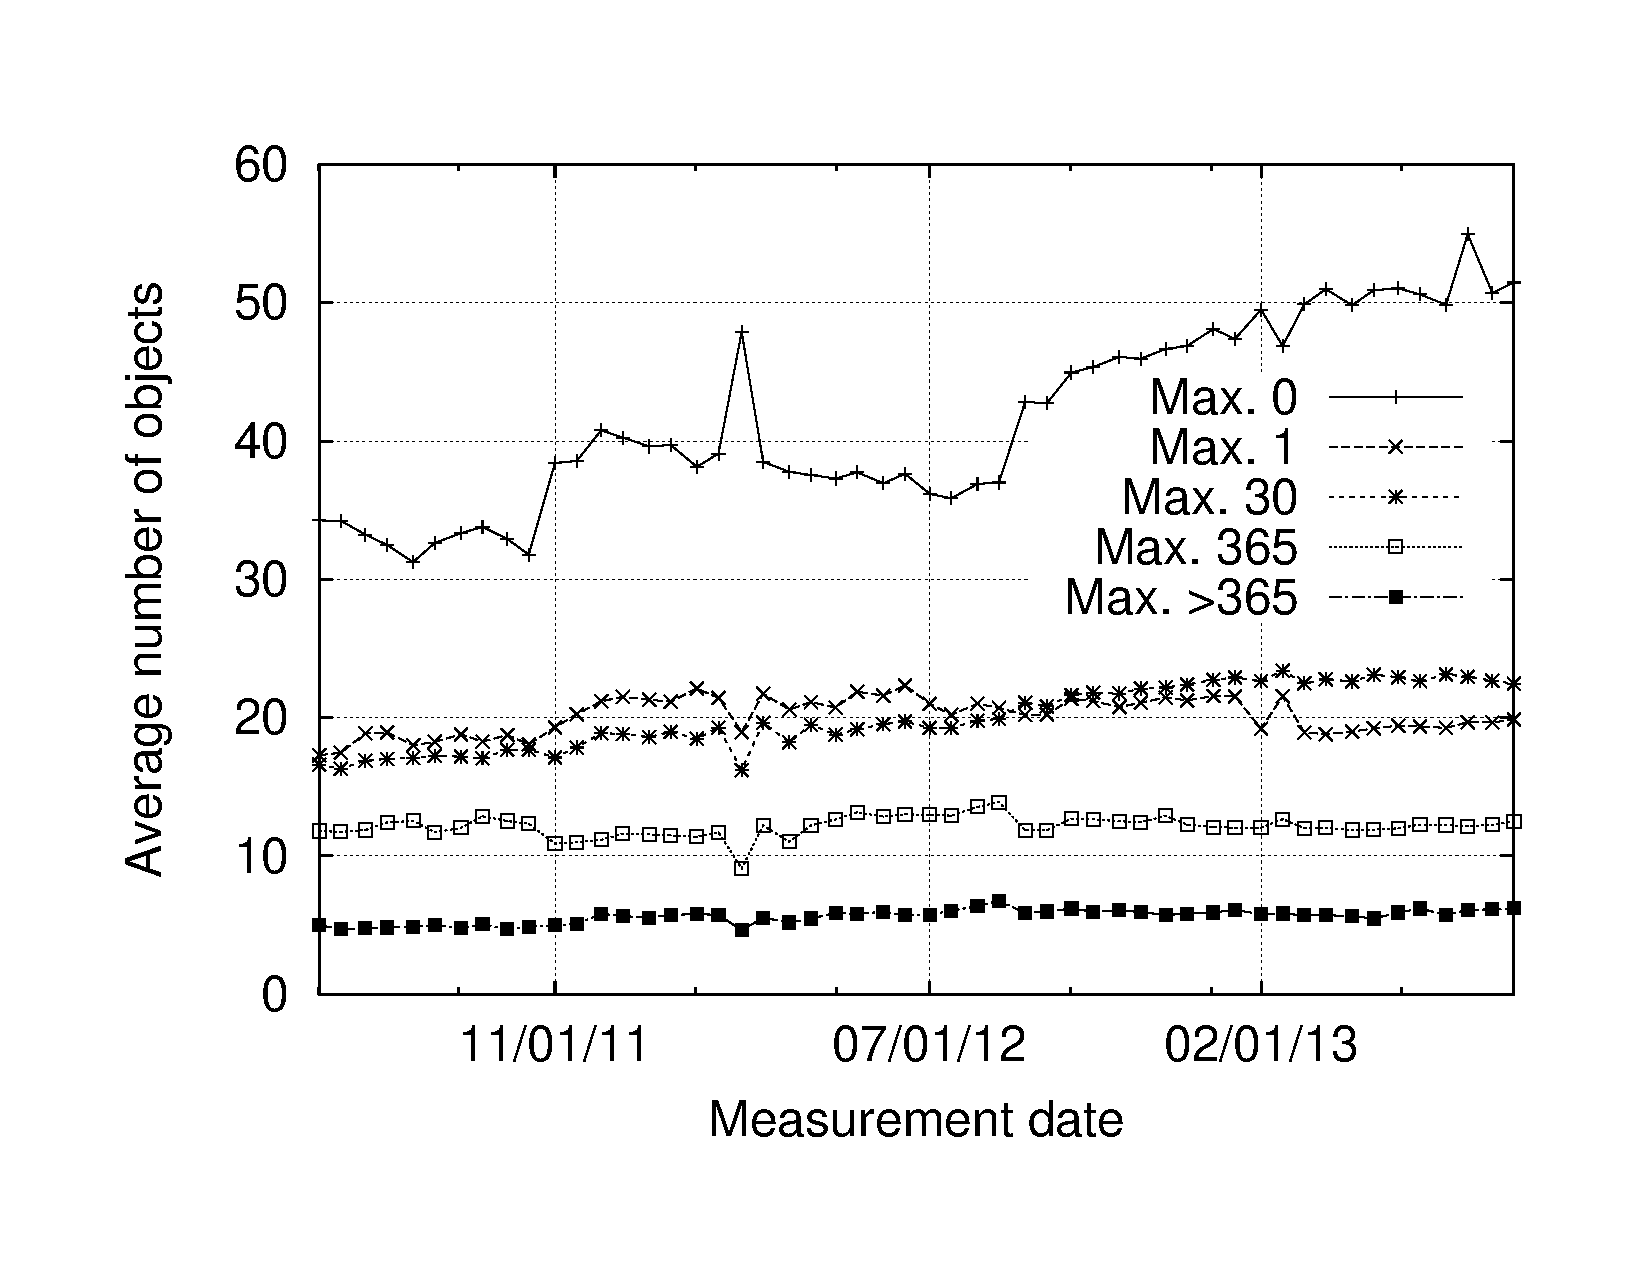
\includegraphics[width=.57\textwidth]{cache_fix}}\\
%	\subfloat[Mobile clients]{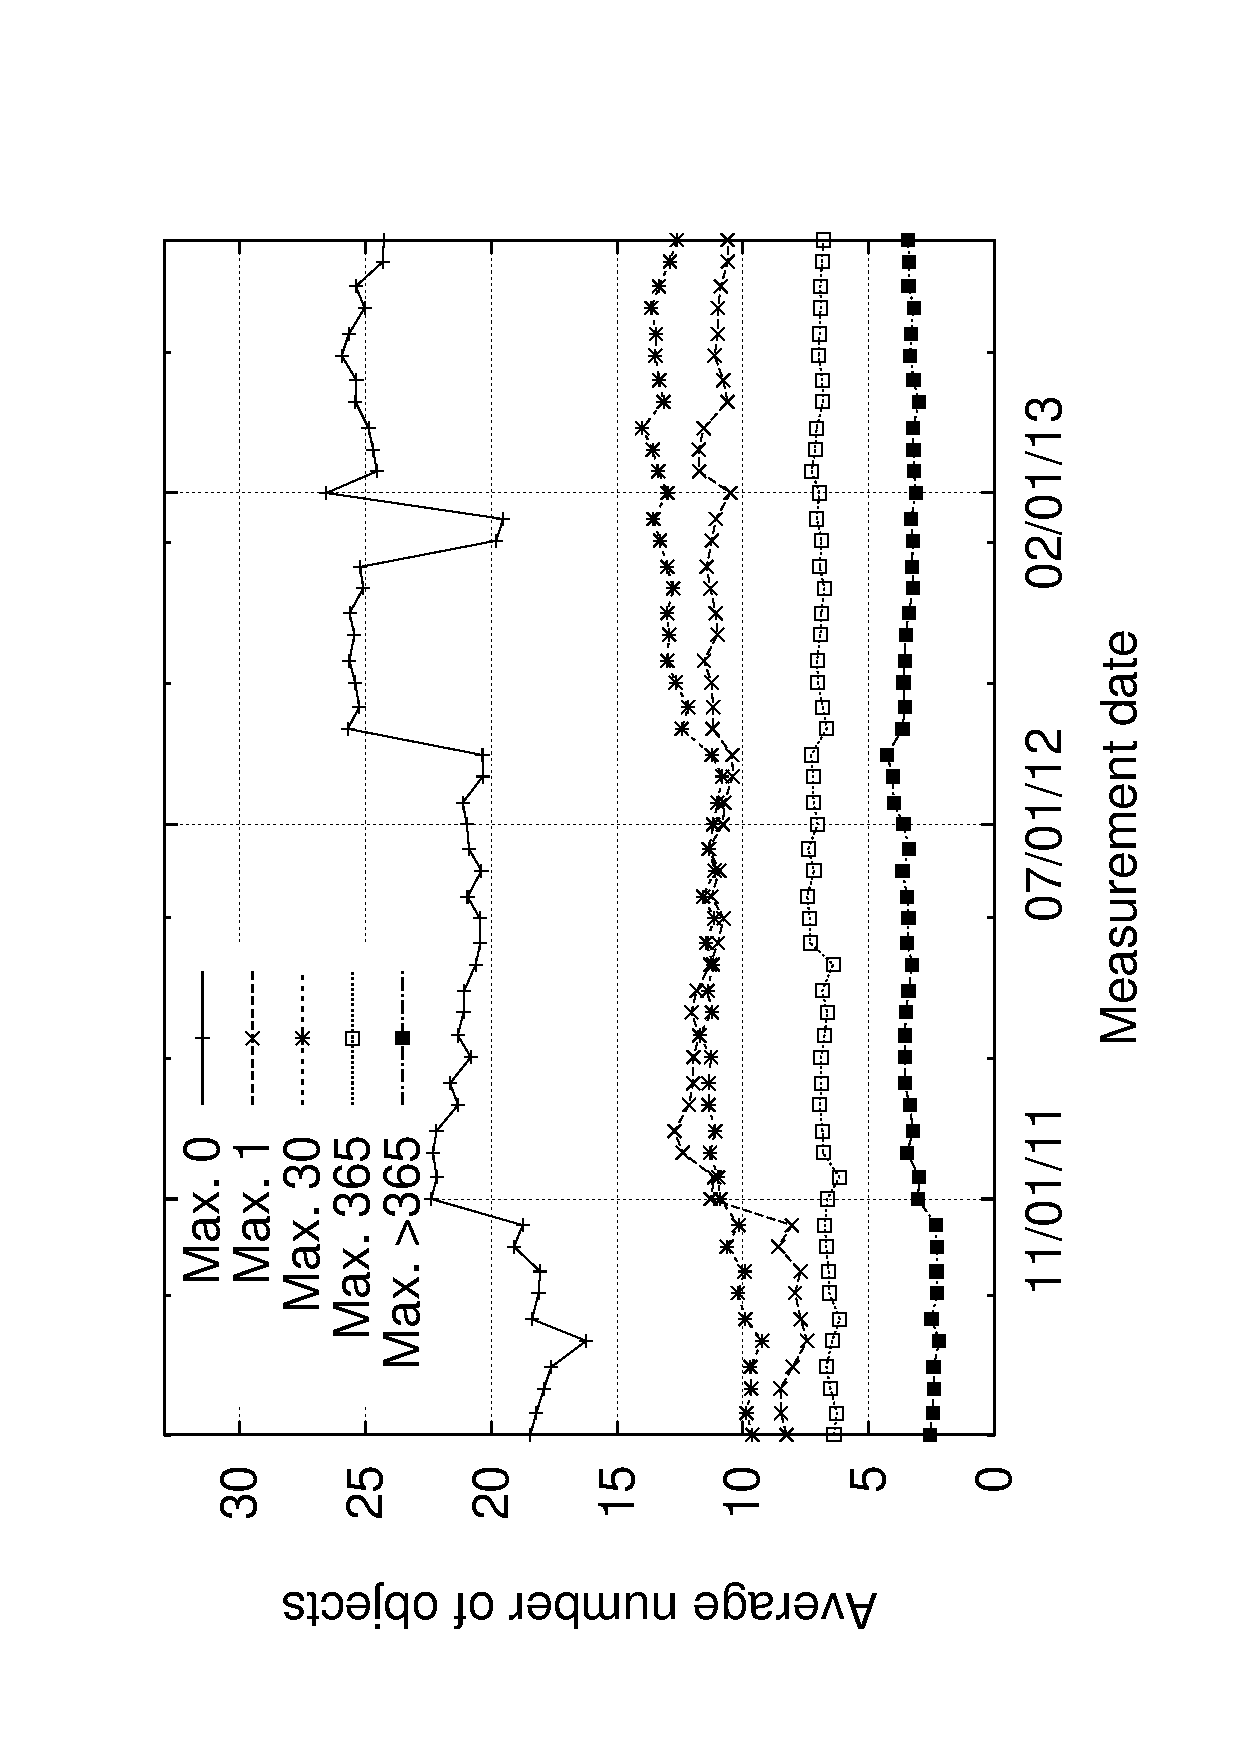
\includegraphics[width=.57\textwidth]{cache_mob}}\\
	\caption{Maximum age of web page objects for desktop and mobile web clients.\label{fig:maxage}}
\end{figure}



\end{document}